% -*- coding: latin1 -*-

\documentclass[12pt,twoside,a4paper]{article}
\usepackage{color}
%\usepackage{ucs}
\usepackage[utf8]{inputenc}
%\usepackage[latin1]{inputenc} 
%\usepackage[T1]{fontenc} 
%\usepackage{pxfonts}
\usepackage{graphicx}
\usepackage{amsmath}
%\usepackage[nonamebreak,round]{natbib}
\usepackage[colorlinks]{hyperref}
\usepackage{fullpage}
\author{Morten N. Åsnes \footnote{No longer at IMR, please contact bjarte.bogstad@imr.no for questions regarding Prost} \\
			Bjarte Bogstad $<$\href{mailto:bjarte.bogstad@imr.no}{bjarte.bogstad@imr.no}$>$\\
        IMR, Bergen, Norway}
\title{Prost Users Guide} 
\bibliographystyle{apalike}



\begin{document}

\newcommand{\console}[1]{\texttt{\textbf{#1}}}
\newcommand{\file}[1]{\texttt{\textbf{#1}}}
\newcommand{\keyword}[1]{\emph{#1}}
\newcommand{\parameter}[1]{\emph{#1}}
\newenvironment{fileformat}{\ttfamily\begin{center}}{\rmfamily\end{center}}
%\renewcommand{\cite}[1]{\citet{#1}}
%\renewcommand{\ref}[1]{\autoref{#1}}

\maketitle \tableofcontents
\newpage
\section{Introduction}
\label{intro}
This document describes the prognosis program Prost (Projections
Stochastic), version 0.1.  The purpose of the program is to perform
stochastic projections using an age structured population model, for
given management rules. The program starts with a given population,
which is then projected into the future and subjected to natural
mortality and fishing. Fishing level is given by a management
rule. Stochastic errors can be added to the initial starting
population (numbers, weight, maturity, etc.), and to the
recruitment. In addition errors can be added to the population before
it is seen by the management rule (assessment error), and to the
decided quota (implementation error).  Each model simulation will thus
give a different realization of the projection.  The model works as
described in 
\hyperlink{skagen}{Skagen et al. (2003)}.  
A yearly time step is used. The following figure
illustrates a single realization of the model.

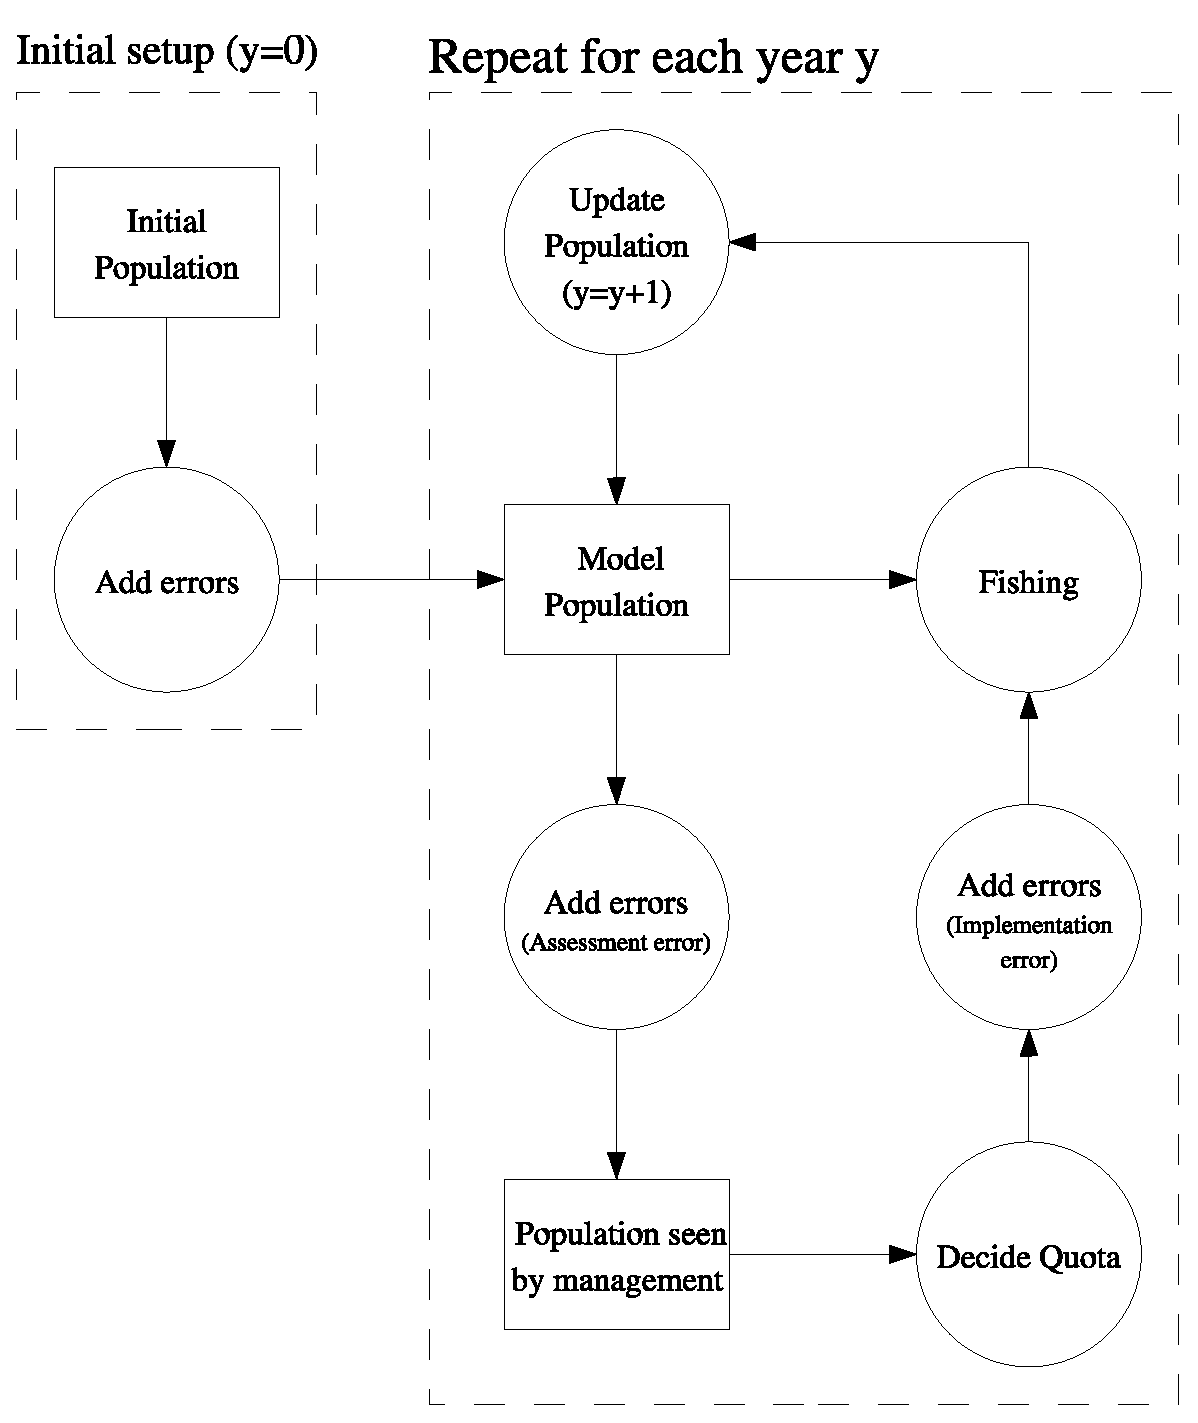
\includegraphics[width=0.8\textwidth]{prostflow}

The program was developed for use in the evaluation of the proposed
harvest control rule for Northeast Arctic cod
\hyperlink{bogstad}{(Bogstad et al. 2004)}, but is generally
applicable for making single-species, single-fleet, single-area
stochastic projections using an age-structured population
model. Weight at age and maturity at age can be density-dependent, and
a variety of harvest control rules can be applied. It is easy to add
more options for density-dependent weight/maturity at age as well as
additional harvest control rules.

The ICES Study group on Long term Advice \hyperlink{ices2004a}{(ICES 2004a)}
 as well as
the ICES Methods Working group \hyperlink{ices2004b}{(ICES 2004b)}
 have discussed existing tools
similar to Prost. Such tools include WGMTERM, ICP, STPR and CS5.


The model does not assume any specific unit in the input and output
files. It is up to the user to make sure that units for numbers and
weight match up. In the manual we assume that numbers are in thousands
and weights are in tons.

\section{Installation}
\label{install}
Prost is written in Java, and can therefore run on any platform where
a Java runtime version is available. 

If you're not developing Java software yourself, it is
sufficient to download the JRE (Java Runtime Environment).  Verify
that you have a suitable Java installation by
typing \console{java -version} in a Dos or Terminal window. The output
should be something like this: 
\begin{verbatim}
java version "1.7.0_45"
Java(TM) SE Runtime Environment (build 1.7.0_45-b18)
Java HotSpot(TM) 64-Bit Server VM (build 24.45-b08, mixed mode)
\end{verbatim}

Please notice that the Java Browser Plugin is not sufficient for running Java Applications like
Prost.

An up
to date JRE can be downloaded at
\url{http://www.oracle.com/technetwork/java/javase/downloads/jre7-downloads-1880261.html}. The
download should be named \emph{jre-7u45-windows-i586.exe} or similar for the 32 bit version,
or \emph{jre-7u45-windows-x64.exe} or similar for the 64 bit version. The download
consists of a setup program, which must then be run to install Java on
your computer.

After running the installer try to run \console{java -version} from a DOS windows 
again to verify that the correct Java version is found.

If for some reason Windows can still not find the installed Java version, you will
have to configure your the windows \emph{Path} environment variable to include the 
path where \console{java.exe} is installed. First, locate directory where \console{java.exe}
is in installed. It should typically be something like \console{c:\textbackslash Program Files\textbackslash Java\textbackslash jre7\textbackslash bin}. 
Now, to add this directory to the system path, click \emph{Start}, then \emph{Control Panel}, then \emph{System}.
Then click \emph{Advanced} and \emph{Environment Variables}.
Now edit the \emph{Path} under \emph{System Variables}, and add the java directory to the end, separated from the previous
entry by a semicolon. The new path should be in effect when you open a new command window.

As an alternative, it is possible to change the path temporarily in a single command window.
In a command windows, type the following: \console{set path=\%path\%;c:\textbackslash Program Files\textbackslash Java\textbackslash jre7\textbackslash bin} (but change the path to reflect where Java is installed on your machine). Now the new path will be in effect only in the current window until it is closed.

Prost comes packaged as a single file called \file{prost.jar}. It is
most convenient to place this file together with the input files in
the directory where you intend to run the program.

\section{Running Prost}
\label{running}
To run Prost, type \console{java -jar prost.jar}. This will read the file
\file{stock.dat}, and start a run. Output will appear in various text files
(\file{.csv} files which can be read into Excel). See Section~\ref{output} 
for more
detail on the output files.  

\subsection{Command Line Options}
\label{options}
To control how many simulations
to perform, add the command line option \console{-i nr\_of\_simulations}. 
For example;
to run 1000 simulations you type: \console{java -jar prost.jar -i 1000}. The
default is 100 simulations.  The option \console{-o} produces very detailed
output to the file \file{out.csv}. When doing many simulations this file will
become very large. It is usually only needed for debugging.

To specify a seed for the random number generator, use the option
\console{-r seed} where seed is an integer.

The option \console{-v} will print some more information to the screen
as the input files are read in. This will be helpful in tracking down any
mistakes in the input files.

It is possible to set the fishing level on the command line with the
option \console{-f flevel}. If this option is used, the given value
will override the \console{FaboveBpa} parameter from the management
file (Section~\ref{management}). 

When this option is used, all output files will have a prefix added to
their name, to distinguish output files from different runs. For
instance;  if the option \console{-f 0.4} is used the summary file
will be named \console{F0.4-summary.csv}.

This option can be useful when one
wants to automate the task of running Prost with different fishing
levels. The script \console{prost.js} can do this on Windows. See
Section~\ref{script} for details on how to use the \console{Prost.js}
script. 

The option \console{-s portnr} specifies that Prost should communicate
with an external program on the specified port. During the simulation
Prost will then read data from this socket each year, 

The data read from the socket is weight in stock, weight in catch,
maturity, and natural mortality. Prost will then write the number of
the start of the next year back over the socket.

\subsection{Scripting}
\label{script}
A script is provided with the Prost distribution, for doing multiple
runs, with different fishing levels. The script will accept all the
usual Prost arguments, but the \console{-f} option is handled
differently. This option is now followed by three values: The smallest
fishing level to use, the largest fishing level, and a step-value. The
script will run Gadget multiple times, starting with the smallest
fishing level, increasing the level by the step value each time, up to
and including the given max level. The script is called
\file{prost.js}, and it will only work on the Windows platform. The
complete syntax is as follows: 

\begin{verbatim}
prost.js -f minf maxf stepf <ordinary prost options>
\end{verbatim}

The script expects the Prost program (\file{prost.jar}) to be in the
same directory as the script is running from, or the directory above
it. If \file{prost.jar} can not be found, the script will exit with an
error message.

\section{Prost Input Files}
\label{input}
All input files are pure text files. They generally consist of keyword
-- value pairs, in a predefined order. Comments can be introduced with
a semicolon. The rest of the line following the semicolon is treated
as a comment.

\subsection{Control file}
\label{control}
The control file must reside in the directory where Prost is started,
and it must be named \file{stock.dat}.  This file specifies the age range and
time span to run the model for. It also lists all the other input
files. An example of the file:
\begin{verbatim}
name               Torsk
firstyear          2003         ; intermediate year
lastyear           2028         ; last prediction year
extrayears         5            ; extra years after lastyear
minage             3            ; recruitment age
maxage             13           ; +group
fbarmin            5
fbarmax            10
bpa                460000
blim               220000
flim               0.49
maxthreshold       20
minthreshold       20
maxf               0.9
summarystart       2004
summaryend         2028
population         pop.dat
recruitment        rec.dat
management         manage.dat
weightandmaturity  density 
file               density.dat
\end{verbatim}

The keywords are explained in Table~\ref{controlkeywords}.

\begin{table}[ht]
\caption{Keywords in control file \label{controlkeywords}}
\begin{tabular*}{\textwidth}{@{\extracolsep{\fill}}llp{9cm}}
%\hline
\textbf{Keyword}      & \textbf{Type} & \textbf{Description} \\
\hline
\keyword{name}      & string  & Name of the stock \\
\keyword{firstyear} & integer & Intermediate year (assessment year) \\
\keyword{lastyear}  & integer & Last year that a quota will be given for \\
\keyword{extrayears} & integer & Extra years needed (for management rule) after \keyword{lastyear} \textbf{(optional)} \\
\keyword{minage} & integer & Minimum age \\
\keyword{maxage} & integer & Maximum age \\
\keyword{fbarmin} & integer & Minimum age for reference F calculation \\
\keyword{fbarmax} & integer & Maximum age for reference F calculation \\
\keyword{bpa} & double & $B_{pa}$ value \\
\keyword{blim} & double & $B_{lim}$ value \\
\keyword{flim} & double & $F_{lim}$ value \\
\keyword{maxthreshold} & double & Threshold for counting a year as having a big increase in quota\\
\keyword{minthreshold} & double & Threshold for counting a year as having a big decrease in quota\\
\keyword{maxf} & double & Maximum fishing mortality \\
\keyword{summarystart} & integer & First year in summary output \\
\keyword{summaryend} & integer & Last year in summary output \\
\keyword{population} & string & Filename for population data \\
\keyword{recruitment} & string & Filename for recruitment function definition \\
\keyword{management} & string & Filename for management rule definition \\
\keyword{weightandmaturity} & string & Option for weight and maturity \\
\keyword{file} & string & Filename for density dependent, or historic weight and maturity \textbf{(optional)} \\
\hline
\end{tabular*}
\end{table}

The model will start some years before the intermediate year because
data from earlier years might be needed for the recruitment
function. And because the management rule may look several years into the
future when setting the quota, the model may also run for several 
years after the
last year. 

The numbers of years to run before $firstyear$ is determined  by the minimum age in
the model. Thus if $minage=2$, the program will require data for two years before
$startyear$. The number of years to run after $lasteyear$ depends on several things.
Firstly, the model must run at least $minage$ years after $lastyears$, this is because of the
way the recruitment function is implemented. Then, if the \keyword{lookahead} management rule is
used, the model must run as many years after $lastyear$ as the \keyword{lookahead} management rule
is set to look into the future. Lastly, there is the keyword \keyword{extrayears} in the control file, 
where the user can specify how many years after $lastyear$ of data are in certain input files.
Thus the number of years to run after $lastyear$ will be the largest value of $minage$, 
$extrayears$, and $years$ (in the \keyword{lookahead} rule). We will call this last year of the
model $Y_N$ in the discussion below.

The $B_{pa}$ value is used only as a trigger point in the constant
F rule (Section~\ref{cfr}) and the lookahead rule (Section~\ref{lookahead}). 
The $B_{lim}$ value is only used for calculating $P(SSB<B_{lim})$ in the summary output. The values $F_{lim}$, 
$maxthreshold$, and $minthreshold$ are also used only for printing.

\subsubsection{Weight And Maturity option}
The keyword \keyword{weightandmaturity} indicates how
weights and maturity are modeled. The option must be one of \keyword{initial},
\keyword{density}, or \keyword{historic}.  If the option is \keyword{initial}, the weight and
maturity comes from the population file, in the format specified
below. If the option \keyword{density} or \keyword{historic} is given, the next line of
the file must give a filename where these options are further
specified. The format for the \keyword{density} option is specified in 
Section~\ref{density}
The \keyword{historic} option is described in Section~\ref{historic}. Note that even
if the \keyword{density} or \keyword{historic} option is given, the initial population
file must still contain weight and maturity.

\subsection{Population File}
\label{population}
The name of the population file is given in the control file. As
mentioned above, all data given here must start in the year
$firstyear-minage$, but depending on which recruitment function is used,
the data before \keyword{firstyear} might not be used.  The following sets of
data must be given (Table~\ref{range}). $Y_i$ is the intermediate year (\keyword{firstyear}), $Y_0$ is
$firstyear-minage$, and $Y_N$ is the last year of the model run as defined above.

\begin{table}[ht]
\caption{Input data type keywords and ranges \label{range}}
\begin{tabular*}{\textwidth}{@{\extracolsep{\fill}}llp{10cm}}
%\hline
\textbf{Keyword}      & \textbf{Range} & \textbf{Description} \\
\hline
[numbers]         & $Y_0 \xrightarrow{} Y_i$ & Population numbers up to and including intermediate year \\

[fishingmortality] & $Y_0 \xrightarrow{} Y_i$ & Fishing mortality up to and including intermediate year \\

[naturalmortality] & $Y_0 \xrightarrow{} Y_N$ & Natural mortality for the whole time period \\

[stockweight]     & $Y_0 \xrightarrow{} Y_N$ & Stock weight for the whole time period \\

[catchweight]     & $Y_0 \xrightarrow{} Y_N$ & Catch weight for the whole time period \\ 

[maturity]        & $Y_0 \xrightarrow{} Y_N$ & Maturity for the whole time period \\

\hline
\end{tabular*}
\end{table}

Each set of data has the following general format:
\begin{verbatim}
[keyword]
expected
<age vector of expected values 1>
...
<age vector of expected values N>
distortion <distortion 1> 
...
distortion <distortion N>
\end{verbatim}

The keyword identifies the type of data. Each age vector gives the
expected value for each age in a given year. Each distortion then
specifies how to draw a random value around the expected. The
distortion format can be one of the following:

\subsubsection{No distortion}
\begin{verbatim}distortion none\end{verbatim}
This will use the expected value directly, no error is added.

\subsubsection{Normally distributed distortion}
\begin{verbatim}
distortion normal
cv <cv age vector>
[bias <Optional bias age vector>]
trunk <truncation>
\end{verbatim}
This will draw from a normal distribution with expected value as
above, and standard deviation $sd=cv \hat{X}$ where $\hat{X}$ is the
expected value.

Optionally bias can be included. This will give a normal distribution 
with mean $\hat{X}+\hat{X}\cdot\mathrm{bias}$. 

\subsubsection{Multivariate lognormally distributed distortion}
\begin{verbatim}
distortion multivariate
covariance <covariance matrix>
\end{verbatim}
This will draw from a multivariate lognormal distribution with
expected value as above, and the given covariance matrix with dimension 
$(maxage-minage+1)*(maxage-minage+1)$. 

\subsection{Recruitment File}
The recruitment functions are defined in a file given by the control
file. Several recruitment functions can be listed, so that for example
a fixed recruitment can be used for the years where data on recruits
are available, and a stock-recruit relationship can be used for other
years. Here is an example of such a file.

\begin{verbatim}
[Recruitment]
generators 2

[RecruitmentGenerator]
firstyear 2004
type fixed
years 2
;       2004    2005   
numbers 308000  664000
error   none 

[RecruitmentGenerator]
firstyear 2006
type  ockham
a     529104
b     224482
error normal
sd    0.2
trunk 2.0
\end{verbatim}
The keyword generators gives the number of recruitment functions. The
recruitment functions are then listed in order. The format is as
follows:
\begin{verbatim}
[RecruitmentGenerator]
firstyear <year>
type <function type>
<function specific input>
<error distribution>
\end{verbatim}

\subsubsection{Recruitment Functions}
\label{recruitment}
The recruitment type can be one of the following:

\subsubsection*{Fixed recruitment}
This reads the recruitment numbers from a file. The recruitment is
then: 
\[R_y=N_y\]
The file format is:
\begin{verbatim}
type fixed
years <nr of years>
numbers <n_1 n_2 ... n_N>
\end{verbatim}
Here N is the number of years that this recruitment function applies
to (see above).

\subsubsection*{Beverton-Holt}
Beverton-Holt gives recruitment according to the following function:
\[R=\frac{a\cdot SSB}{b+SSB}\]
where \emph{SSB} is the spawning stock biomass. The file format for this
function is:
\begin{verbatim}
type bevertonholt
a    <parameter a>
b    <parameter b>
\end{verbatim}

\subsubsection*{Cyclic Beverton-Holt}
The cyclic beverton-holt function has this format:

\begin{verbatim}
type      bevertonholt-cyclic
a         <parameter a>
b         <parameter b>
amplitude 0.43
period    6.57
phase     -1.92
k         0.19
w         4.29
\end{verbatim}

This gives the same recruitment as the beverton-holt function above,
but with a cyclic term included. The recruitment function is thus:
\[
R=f(SSB)e^{amplitude\cdot \sin(\frac{2\pi(year-1946+phase)}{period})
+k(\bar{w}-w)}
\]

where $f(SSB)$ is the normal beverton-holt function:
\[R=\frac{a\cdot SSB}{b+SSB}\]


\subsubsection*{Ricker}
The Ricker recruitment function gives recruitment according to the
following function:
\[R=a\cdot SSB \cdot e^{-b\cdot SSB}\]

The file format is as follows:
\begin{verbatim}
type ricker
a    <parameter a>
b    <parameter b>
[ssb-cutoff <optional parameter ssb-cutoff>]
\end{verbatim}

The parameter \verb+ssb-cutoff+ is optional. If this parameter is given, it 
is used as a maximum $SSB$. If the stock $SSB$ is higher than 
\verb+ssb-cutoff+,
the value of \verb+ssb-cutoff+ will be used instead of $SSB$ in the recruitment
formula above.

\subsubsection*{Ockham}
The ockham recruitment function gives recruitment according to the
following function:
\[
R=\left\{\begin{array}{ll}
    a & \textrm{if} \quad SSB \ge b \\
    \frac{a \cdot SSB}{b} & \textrm{if} \quad SSB < b \\
  \end{array}
  \right.
\]
The file format is then:
\begin{verbatim}
type ockham
a    <parameter a>
b    <parameter b>
\end{verbatim}

\subsubsection*{Cyclic Ockham}
The cyclic ockham function has the following format:
\begin{verbatim}
type      ockham-cyclic
a         <parameter a>
b         <parameter b>
amplitude 0.43
period    6.57
phase    -1.92
k         0.19
w         4.29 
\end{verbatim}
This gives the same recruitment function as Ockham, with a cyclic term
included.
\[
R=f(SSB)e^{amplitude\cdot \sin(\frac{2\pi(year-1946+phase)}{period})
+k(\bar{w}-w)}
\]

Where $f(SSB)$ is the same as the standard Ockham function.

\[
f(SSB)=\left\{\begin{array}{ll}
    a & \textrm{if} \quad SSB \ge b \\
    \frac{a \cdot SSB}{b} & \textrm{if} \quad SSB < b \\
  \end{array}
  \right.
\]
$\bar{w}$ is here the mean weight in the spawning stock.

This recruitment function is further described in 
\hyperlink{bogstad}{Bogstad et al. (2004)}.

\subsubsection{Recruitment Error}

For all recruitment functions an error distribution must be
specified (it can be set as \keyword{none} if no error is to be
added). The error distribution is specified using one of the following
formats. 

\subsubsection*{Normal distribution}
\begin{verbatim}
error normal
cv    <coefficient of variance>
[bias <Optional bias age vector>]
trunk <truncation>
\end{verbatim}
This gives an error ($\varepsilon$) drawn from a normal distribution
with $mean=0.0$ and $sd=cv$. $\varepsilon$ is truncated to be
in the range $[-trunk\cdot cv \rightarrow trunk\cdot cv]$. If $R$ is
one of the recruitment functions in Section~\ref{recruitment} the
number of recruits is then $R'=R+R\cdot \varepsilon$.

Optionally bias can be included. This gives the number of recruits as
$R'=R+R\cdot\mathrm{bias}+R\cdot \varepsilon$.


\subsubsection*{Lognormal distribution}
\begin{verbatim}
error lognormal
cv    <cv on a log scale>
[bias <Optional bias age vector>]
trunk <truncation>
\end{verbatim}
This gives an error ($\varepsilon$) drawn from a lognormal distribution
with $mean=0.0$ and $sd=cv$. $\varepsilon$ is truncated to be
in the range $[-trunk\cdot cv \rightarrow trunk\cdot cv]$. The
number of recruits is then $R'=R{\cdot}e^{\varepsilon}$.

Optionally bias can be included. This gives the number of recruits as
$R'=R\cdot\mathrm{bias}+R{\cdot}e^{\varepsilon}$.

\subsubsection*{No error}
\begin{verbatim}
error none
\end{verbatim}
This gives no error added to the recruitment. $R'=R$.

\subsubsection{Special recruitment functions}

In this section we list ad-hock recruitment functions which have been added for
specific situations. They are not meant to be general.

\subsubsection*{Cyclic Haddock}
This is a special recruitment function intended used for haddock. It
gives recruitment according to the following 7-year cycle: 
\begin{itemize}
\item Four years with \emph{low} recruitment.
\item One year with \emph{good} recruitment.
\item Probability $p$ of a year with \emph{outstanding} recruitment, \\
      or a year with \emph{good} recruitment with probability $1-p$.
\item One year with \emph{good} recruitment.
\end{itemize}

For the years with low recruitment a Ricker function is used. A ricker
function is also used for the good years, and an Ockham function is used
for the outstanding year. Thus three sets of recruitment parameters
must be given; for the Ricker function in low years, for the ricker
function in good years, and for the Ockham function in Outstanding
years. In addition and error function must be specified after each of
these recruitment functions. The Input formats are the same as
described for the Ricker function, Ockham function, and error functions
described in the previous sections. The complete format for the cyclic
haddock recruitment is thus as follows:
\begin{verbatim}
type haddock-cyclic
low-recruitment
  a <parameter a for ricker>
  b <parameter b for ricker>
  [ssb-cutoff <optional parameter ssb-cutoff for ricker>]
  error <error type>
  <parameters for error>
good-recruitment
  a <parameter a for ricker>
  b <parameter b for ricker>
  [ssb-cutoff <optional parameter ssb-cutoff for ricker>]
  error <error type>
  <parameters for error>
outstanding-recruitment
  p <probability of outstanding recruitment>
  a <parameter a for ockham>
  b <parameter b for ockham>
  error <error type>
  <parameters for error>
\end{verbatim}


\subsection{Management File}
\label{management}
The management file defines the management rule to use for setting the
fishing quota. It also specifies how the real model is distorted
before the managers see it, and how the decided quota is distorted
before it is fed back to the real model. The format is as follows:
\begin{verbatim}
[ManagementDistortions] 
ImplementationError distortion none
InputNumbers        distortion none 
InputFishing        distortion none 
Recruitment         distortion none

[ManagementRule]
type <management rule>
<input for management rule>
\end{verbatim}

The format for distortion is the same as for the population file
(Section~\ref{population}). 
The rule type can be one of  \keyword{constantf},  
\keyword{tac}, or \keyword{lookahead}.
Let \emph{F} be the \emph{reference F} (arithmetic average over the age range
$fbarmin-fbarmax$) and $S_a$ the selection age vector. The
\emph{fishing mortality} for age \emph{a} is then given by:

\[
F_a=\displaystyle F\cdot S_a\cdot \frac{\displaystyle\sum_{a=\mathrm{fbarmin}}^{\mathrm{fbarmax}}{S_a}}{(\mathrm{fbarmax} - \mathrm{fbarmin} + 1)}
\]

All the rules will calculate a quota in tons for year $y+1$. We then
use the selection pattern (from the input file) to find the
appropriate fishing level that gives this quota. We then use this
fishing level to calculate catch in numbers for year $y+1$. This
catch in numbers is then fed back to the model and used for fishing in
year $y+1$ after possibly being distorted.  The ImplementationError
above decides how the quota is distorted before it is fed back into
the model as fishing mortality.



\subsubsection{Constant F Rule}
\label{cfr}
For the \emph{constant F rule} the format is:
\begin{verbatim}
type         constantF
Selection    <selection age vector>
FaboveBpa    <F level above Bpa>
[Fmin        <Optional minimum F level>]
[FlowRec     Optional keyword enable adjustment of F at low recruitment>]
[LowRec      <LowRec> Recruitment belowe this number is considerd poor.]
[LowYears    <years> How many years of recruitment to consider]
[Freduction  <factor> At low recruitment multiply F by this factor]
[HistoricRec <recruitment vector> Historic recruitment before first year]
Maxinc       <Max increase in quota from last year>
Maxdec       <Max decrease in quota from last year>
MaxTAC       <Max allowed catch in weight>
FirstYearTAC <quota for intermediate year>
FbelowBpa    <function type>
\end{verbatim}


The \keyword{fbelowpa} function is one of the keyword \keyword{flat},
\keyword{low}, or \keyword{linear}. The formats are:

\begin{verbatim}
flat
\end{verbatim}
Which gives $F=F_{target}$ when $SSB<B_{pa}$

\begin{verbatim}
low
Flow <flevel>
\end{verbatim}
Which gives $F=F_{low}$ when $SSB<B_{pa}$

\begin{verbatim}
linear
Bzero <Bzero>
\end{verbatim}
Which gives $F=\frac{(SSB-B_{zero})\cdot F_{aboveBpa}}{B_{pa}-B_{zero}}$ 
when $B_{zero} < SSB<B_{pa}$ and $F=0$ when $SSB<B_{zero}$.

If $SSB(y+1)>B_{pa}$ and $SSB(y)>B_{pa}$, the quota is constrained by the limits
on year-to-year change indicated by the keywords \keyword{maxinc} and \keyword{maxdec}:
If the quota is more than \keyword{maxinc} percent larger than last years
quota, or more than \keyword{maxdec} percent less, we adjust the quota
to be within \keyword{maxdec} and \keyword{maxinc} percent of last
years quota.   

If \keyword{firstyeartac} is $-1$ the \keyword{maxinc} and \keyword{maxdec}
 values are not used for setting the quota in year $y+1$. If \keyword{firstyeartac} is positive
the value is used when applying the \keyword{maxinc} and \keyword{maxdec} check in year $y+1$.

The $MaxTAC$ parameter makes it possible to 
use this option to apply a constant F rule with a catch ceiling.

If the \keyword{FlowRec} is present, the following keywords must also be present in this exact order:
\begin{verbatim}
FlowRec
LowRec      <LowRec>
LowYears    <years>
Freduction  <factor>
HistoricRec <recruitment vector>
\end{verbatim}
This option will reduce F when the stock goes through several consecutive years with poor recruitment.
The value Lowrec gives the level the average recruitment has to fall below to be considered poor. 
The value LowYears specifies over how many years this average recruitment is calculated.’
The value \keyword{Freduction} gives a factor by which the target F level will be multiplied in case of 
poor recruitment.
The recruitment vector gives recruitment values for the years before the intermidiate year in the model.
There must be $LowYears-1$ values given.

If the optional \keyword{Fmin} is given, it must be followed by an F value. Whenever there is a year where the fishing level is below this \keyword{Fmin} level, except in years where $SSB < Bpa$, F will be adjusted up to the Fmin level. Because the
\keyword{constantF} rule applies a constant F level, the \keyword{Fmin} option is only
useful if some other constrains that can potentially reduce F are also in use.

\emph{It is not advised to use both the \keyword{FlowRec} and \keyword{Fmin} options at the same time.
A warning will be given if you do so.}

\subsubsection{Lookahead Rule}
\label{lookahead}

The Lookahead rule is a generalization of the 3-year rule. The 3-year rule was suggested 
by the Joint Norwegian-Russian Fisheries Commission in 2002,
as a way of stabilizing the quota for the Northeast Arctic cod and haddock stocks by looking
more than one year into the future. 

The format for the lookahead rule is similar to the format for the \keyword{constantF} rule (\ref{cfr}) with a few changes:
\begin{verbatim}
type         lookahead
[years       <N> Optional specification of how many years to simulate]
selection    <selection age vector>
FaboveBpa    <F level above Bpa>
[Fmin        <Optional minimum F level>]
[FlowRec     Optional keyword enable adjustment of F at low recruitment>]
[LowRec      <LowRec> Recruitment below this number is considered poor.]
[LowYears    <years> How many years of recruitment to consider]
[Freduction  <factor> At low recruitment multiply F by this factor]
[HistoricRec <recruitment vector> Historic recruitment before first year]
Maxinc       <max increase in quota from last year in percent>
Maxdec       <max decrease in quota from last year in percent>
MaxTAC       <max allowed catch in weight>
Firstyeartac <quota for intermediate year>
[MaxChangeRuleVariant <Optional keyword>]
Fbelowpa     <function type>
\end{verbatim}

The Optional keyword \keyword{years} specifies how many years to simulate forward when
deciding on the quota. If this keyword is omitted, it will be set to 3 years.

When the \emph{Lookahead Rule} is used in year $y$ to set the fishing quota for
year $y+1$, we first simulate N years forward from these starting values, with a
fishing level dependent on SSB(y+1) in the same way as in the \emph{constant F rule}. 

We set the quota for year $y+1$ as the average of the catch in tons in
the years $y+1$, $y+2$, ... ,$y+n$ from the simulation we did. 

If $SSB(y+1)>B_{pa}$ and $SSB(y)>B_{pa}$, the quota is constrained by the limits
on year-to-year change in the same way as for the \emph{constant F rule}. But if the
optional keyword \keyword{MaxChangeRuleVariant} is specified, the year-to-year change 
is only constrained if $SSB(y')>B_{pa}$ for all the years $y$, $y+1$, $y+2$ and $y+n$.

If weight in catch is density-dependent (\ref{density})
and the \emph{3-year rule} is used, The \emph{weight at age in the catch} used by
the rule in year $y+1$ is also used int the remaining years.

The options \keyword{Fmin} and \keyword{FlowRec} work as for the \keyword{constantF} rule, and are described in section \ref{cfr}

\subsubsection{3-year Rule}
\label{3yr}

$\\$

\textbf{The 3-year rule has been deprecated, please use the lookahead rule instead.}

$\\$

The 3-year rule is a way of stabilizing the quota by looking more than one year
ahead.  It was suggested by the Joint Norwegian-Russian Fisheries Commission in 2002,
for the Northeast Arctic cod and haddock stocks.

The format for the 3-year rule is:
\begin{verbatim}
type         3year
selection    <selection age vector>
FaboveBpa    <F level above Bpa>
Maxinc       <max increase in quota from last year in percent>
Maxdec       <max decrease in quota from last year in percent>
MaxTAC       <max allowed catch in weight>
Firstyeartac <quota for intermediate year>
[MaxChangeRuleVariant <Optional keyword>]
Fbelowpa     <function type>
\end{verbatim}

When the \emph{3-year Rule} is used in year $y$ to set the fishing quota for
year $y+1$, we first simulate 3 years forward from these starting values, with a
fishing level dependent on SSB(y+1) in the same way as in the 3-year rule. 

We set the quota for year $y+1$ as the average of the catch in tons in
year $y+1$,$y+2$, and $y+3$ from the simulation we did. 

If $SSB(y+1)>B_{pa}$ and $SSB(y)>B_{pa}$, the quota is constrained by the limits
on year-to-year change in the same way as for the \emph{constant F rule}. But if the
optional keyword \keyword{MaxChangeRuleVariant} is specified, the year-to-year change 
is only constrained if $SSB(y')>B_{pa}$ for all the years $y$, $y+1$, $y+2$ and $y+3$.

If weight in catch is density-dependent (\ref{density})
and the \emph{3-year rule} is used, The \emph{weight at age in the catch} used by
the rule in year $y+1$ is also used for the years $y+2$ and $y+3$.

\subsubsection{Tac Rule}
\label{tacr}
For the \emph{Tac Rule} the format is:
\begin{verbatim}
type tac
Selection <selection age vector>
maxF      <maximum F level>
TAC
<y_1> <Tac_1>
<y_2> <Tac_2>
.     .
.     .
.     .
<y_n> <Tac_n>
\end{verbatim}
With this rule you simply specify in the input file the quota in tons
for each year.  The $maxF$ parameter makes it possible to 
use this option to apply a fixed F rule with a catch ceiling.

\subsection{Density dependent processes}
\label{density}
In this file, you can specify that various processes in the model will
be density dependent. The processes are growth (stock weights and
catch weights), maturity, and cannibalism. In all cases the age range
the process will apply to can be restricted to a subrange of the full
age range in the stock. There is also an option to give minimum and
maximum values for each age group.

The functional forms for growth, and the first maturity variant are
described in \hyperlink{bogstad}{Bogstad et al. (2004)}. 
All the functions are further described below.

The format for density dependent processes is:
\begin{verbatim}
stockweight <yes or no>
<if yes, additional input for stockweight>

catchweight <yes or no>
<if yes, additional input for catchweight>

maturity <yes or no>
<if yes, additional input for maturity>

cannibalism <yes or no>
<if yes, additional input for cannibalism>
\end{verbatim}

\subsubsection{Growth (stockweight and catchweight)}

The following function is used for weight in the stock:
\[ws_{a,y}=\alpha_a TSB_{y-1}+\beta_a\]
For weight in the catch this function is used:
\[wc_{a,y}=\alpha_a ws_{a,y}+\beta_a\]

Both \emph{stockweight} and \emph{catchweight} uses the following
format:
\begin{verbatim}
minage      <minage>
maxage      <maxage>
alpha       <alpha parameter age vector>
beta        <beta parameter age vector>

limit                          ; optional limit  
  min  x1 ... xn               ; minimum value for each age (optional)
  max  y1 ... yn               ; maximum value for each age (optional)
\end{verbatim}


\subsubsection{Maturity}
The maturation process can use one of two different functions.
The \keyword{function} keyword followed by \emph{densitydependent} or
\emph{weightdependent} selects which function to use.

The \emph{densitydependent} function is:
\[
P_{a,y}(TSB)=\frac{1}
             {1+e^{-\alpha(\gamma a-\kappa-TSB_{y-1})}}
\]
Where TSB denotes total stock biomass. 

The \emph{weightdependent} function is:
\[
P_{a,y}(ws_{a,y})=\frac{1}
                {1+e^{-\lambda_a(ws_{a,y}-w_{{50},a})}}
\]

The format for the \emph{densitydependent} function is:
\begin{verbatim}
function    densitydependent
minage      <minage>
maxage      <maxage>
alpha       <alpha parameter>  
kappa       <kappa parameter>  
gamma       <gamma parameter>  

limit                          ; optional limit  
  min  x1 ... xn               ; minimum value for each age (optional)
  max  y1 ... yn               ; maximum value for each age (optional)
\end{verbatim}

The format for the \emph{weightdependent} function is:
\begin{verbatim}
function    weightdependent
minage      <minage>
maxage      <maxage>
lambda      <lambda parameter age vector>
w50         <w50 parameter age vector>

limit                          ; optional limit  
  min  x1 ... xn               ; minimum value for each age (optional)
  max  y1 ... yn               ; maximum value for each age (optional)
\end{verbatim}

\subsubsection{Cannibalism}
The cannibalism process can use one of two different functions.
The \keyword{function} keyword followed by \emph{ssblag3} or
\emph{biomass6and7} selects which function to use.
The \emph{ssblag3} function is:
\[
  {M2}_{y,a}=\alpha_a{SSB}_{y-3}+\beta_a
\]
Where SSB denotes spawning stock biomass. 
The \emph{biomass6and7} function is:
\[
  {M2}_{y,a}=\alpha_a(N_{y,6}W_{y,6}+N_{y,7}W_{y,7})+\beta_a
\]

Both the \emph{ssblag3} and \emph{biomass6and7} function uses the following
input format:
\begin{verbatim}
function    <ssblag3 or biomass6and7>
minage      <minage>
maxage      <maxage>
alpha       <alpha age vector>
beta        <beta age vector>   

limit                          ; optional limit  
  min  x1 ... xn               ; minimum value for each age (optional)
  max  y1 ... yn               ; maximum value for each age (optional)
\end{verbatim}


\subsection{Historic weight and maturity}
\label{historic}
In this file, you can specify how stock weights, catch weights, 
and maturity are drawn from historic time series. The format is:

\begin{verbatim}
numberofyears <n>

stockweight <yes or no>
file <file with historic stockweights>

catchweight <yes or no>
file <file with historic catchweights>

maturity <yes or no>
file <file with historic maturities>
\end{verbatim}

Each of these files has the following format:

\begin{verbatim}
historicdata
d1,1 ... d1,a
 ...
dy,1 ... dy,a
\end{verbatim}

where y is the number of years with historic data, and a is the number of 
age groups.

\section{Prost Output Files}
\label{output}
Summary output is written to the file \file{summary.csv}.  More detailed
output for individual variables can be found in \file{fishing.csv},
\file{distortedfishing.csv}, \file{recruit.csv}, \file{catch.csv}, 
\file{ssb.csv}, and
\file{tsb.csv}. On the file \file{rule.csv} it is indicated how often the various 
segments of a HCR are activated. 

The file \file{out.csv} gives very detailed output, and can become quite
large. It is most useful for diagnostic purposes.  All the output
files are written as comma separated values (\file{.csv}) and can thus be
imported into \emph{Excel} or other spreadsheets for further processing.

\section{Suggested extensions}
\label{extensions}

\begin{itemize}

%\item Distortion and recruitment error: The mean should be included as an extra parameter, in order to allow for bias. 

\item Extend the $linear$ option in the $fbelowpa$ function with a new parameter $Fzero$.
The formula for F will then be: 
$F=Fzero+\frac{(SSB-B_{zero})\cdot F_{aboveBpa}}{B_{pa}-B_{zero}}$ 
when $B_{zero} < SSB<B_{pa}$ and $F=Fzero$ when $SSB<B_{zero}$.

%\item The 3-year rule option should be extended/changed  to account for the modification suggested by 
%the Joint Norwegian-Russian Fisheries Commission in 2004, i.e. the
%maximum percentage change from year y to year y+1 should only be applied when
%$SSB > B_{pa}$ in all the years y-1..y+3.  

\item Extending the historic option so that fishing pattern and natural mortality also can be drawn 
from historic times series.

\item Allow for a non-zero proportion of F and M before spawning.

\item Allow for the maximum increase/decrease in TAC from year to year to be given in biomass in addition to
as a percentage.

\end{itemize}

\section{References}

\newenvironment{mybib}{\setlength{\parindent}{0in}\setlength{\parskip}{2ex}}{}

\begin{mybib}

\hypertarget{bogstad}{}
Bogstad, B., Aglen, A., Skagen, D. W., Åsnes, M.N., Kovalev, Y., Yaragina, 
N. A. 2004. \emph{Evaluation of the proposed harvest control rule for
Northeast Arctic cod}. Pp. 396-417 in Report of the ICES Arctic Fisheries Working Group,
Copenhagen 4-13 May 2004. ICES C.M. 2004/ACFM:28, 483 pp.

\hypertarget{ices2004a}{}
ICES 2004a. \emph{Report of the ICES Study Group for Long Term Advice}, 
Copenhagen 23-27 February 2004. ICES C.M. 2004/ACFM:16, 38 pp.

\hypertarget{ices2004b}{}
ICES 2004b. \emph{Report of the ICES Working Group on Fish Stock Assessment 
Methods}, Lisbon 11-18 February 2004. ICES C.M. 2004/D:03, 232 pp.

\hypertarget{skagen}{}
Skagen, D. W., Bogstad, B., Sandberg, P., and Røttingen, I. 2003. 
\emph{Evaluation of candidate management plans, with references to North-east 
Arctic cod}. ICES C.M. 2003/Y:03, 19pp.



\end{mybib}

\end{document}
